\startchapter{Objects, Event Selections and Triggers}
\label{chapter:objects}

This chapter describes the physics objects which are reconstructed on an event-by-event basis using collision data from the ATLAS detector and used in this DM search. It also discusses the triggers and event selection cuts which are applied to define the subsets of collision data and MC simulated data, also known as ``analysis regions", which are used for the search. 

\section{Object Definitions}
\label{ap:object_defs}

The goal of the ATLAS detector is to identify particles that are produced by the proton-proton collisions that take place in the centre of the detector, and to reconstruct their kinematic properties. The particle identification and reconstruction is performed using various collections of measured signals in the detector sub-systems, which are broadly referred to as ``physics objects" \cite{physics_objects_atlas_2013}. The physics objects used to reconstruct all particles considered in this search are described in the following sections.

\subsection{Charged Leptons}

The final state charged lepton produced from the leptonic decay of a \(W\) in the DH model could with approximately equal probability be an electron, a muon or a tau. Electrons are stable and as such do not decay before depositing their energy in the ATLAS detector. This allows them to be reconstructed directly using information from the inner tracker and the EM calorimeter, as discussed in Sections \ref{sec:inner_detector} and \ref{sec:EM_calo}. Muons are unstable and will ultimately decay to a \(\nu_\mu\) and a \(e\bar{\nu}_e\) pair via a virtual \(W\) boson mediator, as shown in Figure \ref{fig:muon_decay}. However, their mean lifetime of 2.2\(\mu s\), which is the average time after they are produced before they undergo the decay to \(\nu_\mu+e\bar{\nu}_e\), is long enough that muons do make it through the ATLAS detector before they decay, and are reconstructed using information from the inner tracker and the muon spectrometer, as discussed in Sections \ref{sec:inner_detector} and \ref{sec:EM_calo}. Muons are only able to decay to a \(e\bar{\nu}_e\) pair because any other particles that the virtual \(W\) could in principle decay to are too massive to be produced from the initial \(106~\MeV\) rest mass energy of the muon. 

\begin{figure}[hp]
	\centering
	\begin{subfigure}[t]{0.49\textwidth}
	\centering
	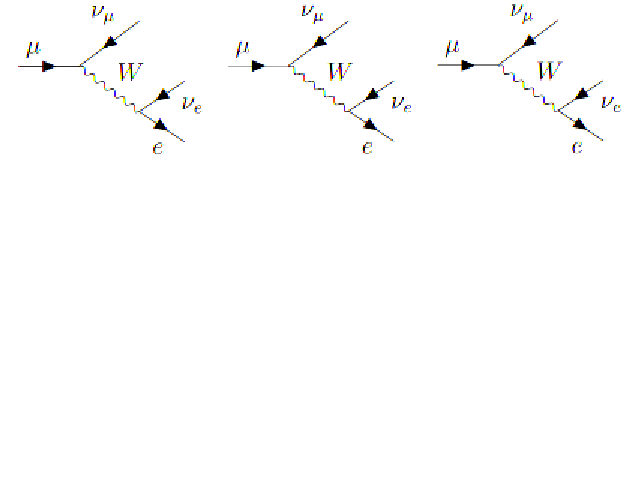
\includegraphics[width=0.5\textwidth]{Figures/5/mu_decay.pdf}
%		 \begin{tikzpicture}
%		 	\begin{feynman}
%		 		\vertex (a1); %mu
%
%		 		\vertex at ($(a1) + (1cm, 0)$) (b1); % decay to W+nu_mu
%				
%		 		\vertex at ($(b1) + (1, 0.75)$) (c1); %nu_mu
%				\vertex at ($(b1) + (1, -0.75)$) (c2); %W
%				
%				\vertex at ($(c2) + (0.75, 0.5)$) (d1); % nu_e
%				\vertex at ($(c2) + (0.75, -0.5)$) (d2); % e
%
%		 		\diagram* {
%		 		  (a1) -- [fermion, edge label=\(\mu\), near start] (b1),
%		 		  (c1) -- [fermion, edge label'=\(\nu_\mu\), near start] (b1) -- [boson, edge label=\(W\)] (c2),
%		 		  (d1) -- [fermion, edge label=\(\nu_e\), near start] (c2) -- [fermion, edge label'=\(e\), near end] (d2),
%		 		};
%		 	\end{feynman}
%		 \end{tikzpicture}
	\caption{Muon decay}
	\label{fig:muon_decay}
	\end{subfigure}
	\begin{subfigure}[t]{0.49\textwidth}
	\centering
	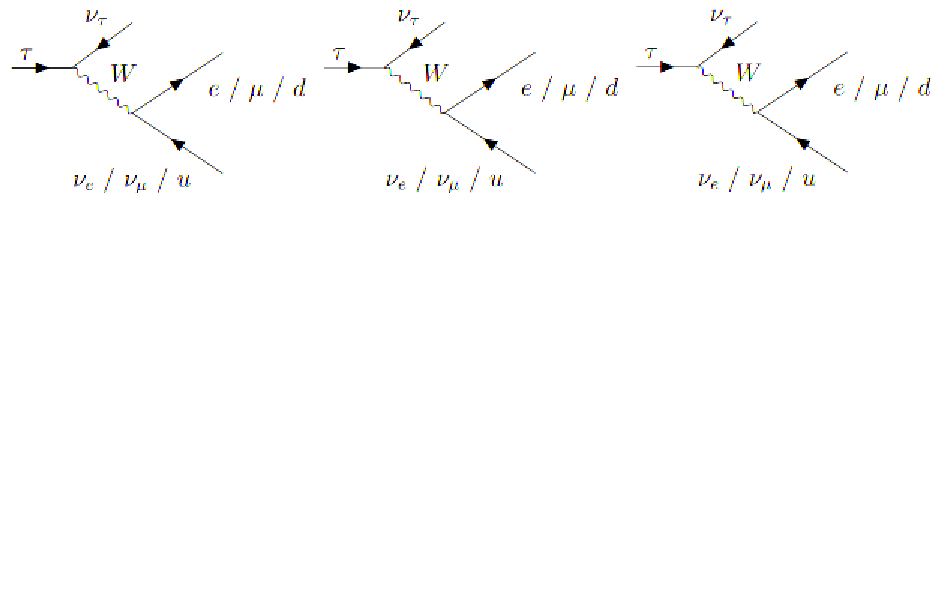
\includegraphics[width=0.75\textwidth]{Figures/5/tau_decays.pdf}
%		 \begin{tikzpicture}
%		 	\begin{feynman}
%		 		\vertex (a1); %tau
%
%		 		\vertex at ($(a1) + (1cm, 0)$) (b1); % decay to W+nu_tau
%				
%		 		\vertex at ($(b1) + (1, 0.75)$) (c1); %nu_tau
%				\vertex at ($(b1) + (1, -0.75)$) (c2); %W
%				
%				\vertex at ($(c2) + (1.5, -1)$) (d1); % nu_e / nu_mu / u / d
%				\vertex at ($(c2) + (1.5, 1)$) (d2); % e / mu / d / u
%
%		 		\diagram* {
%		 		  (a1) -- [fermion, edge label=\(\tau\), near start] (b1),
%		 		  (c1) -- [fermion, edge label'=\(\nu_\tau\), near start] (b1) -- [boson, edge label=\(W\)] (c2),
%		 		  (d1) -- [fermion, edge label={\(\nu_e\) / \(\nu_\mu\) / \(u\)}, near start] (c2) -- [fermion, edge label'={\(e\) / \(\mu\) / \(d\)}, near end] (d2),
%		 		};
%		 	\end{feynman}
%		 \end{tikzpicture}
	\caption{Tau decay}
	\label{fig:tau_decay}
	\end{subfigure}
	\caption{Decay mechanisms for muons and taus}
	\label{fig:lepton_decays}
\end{figure}

Due to their relatively large mass of 1.8 \GeV, taus can decay either leptonically to \(e\bar{\nu}_e\) or \(\mu\bar{\nu}_\mu\), or hadronically to \(d\bar{u}\), as shown in Figure \ref{fig:tau_decay}, and their decays proceed with a much shorter mean lifetime compared with the muon of 0.3ps. Because of this relatively short lifetime, taus will decay before passing through the ATLAS detector, and as such it is their leptonic or hadronic decay products that are actually measured in the detector. As will be discussed in Section \ref{sec:evt_selections} below, the selections applied for this analysis require that events have exactly one electron or muon in the final state in order to be considered for the search. As a result, the search is sensitive to \(s\rightarrow WW\) decays in which the leptonically decaying \(W\) decays to \(\tau\nu_\tau\) only in the case where the \(\tau\) decays leptonically to produce a single energetic electron or muon in the final state, which occurs with a 35\% branching fraction.

\subsubsection{Electrons}

As discussed in Section \ref{sec:EM_calo}, electron objects are reconstructed from clusters of energy deposits in the electromagnetic calorimeter that are associated with tracks in the inner detector, and calibrated to the EM scale. Detailed information about electron reconstruction, identification, and calibration can be found in Refs.~\cite{ATL-PHYS-PUB-2017-022}, \cite{PERF-2017-01} and \cite{PERF-2017-03}. To accommodate the differing needs of the various studies which make use of electron objects, ATLAS reconstructs these objects at several levels of identification and isolation efficiency, where these different efficiency levels are referred to as ``working points", and are typically referred to as variants of \emph{Loose}, \emph{Medium} and \emph{Tight} for reasons that will be discussed in the following paragraphs.

The identification efficiency refers to the probability that an electron passing through the detector will be correctly reconstructed and identified as such. In general, higher efficiency is achieved by loosening electron identification criteria, and comes at the cost of increased background acceptance. Increased background acceptance means that reconstructed objects have a higher probability of being incorrectly identified as having originated from an electron. 

Electron isolation tackles a slightly different, though related, challenge in comparison with identification. The goal of isolation is to separate the so-called ``prompt" electrons that are produced from the primary decay processes of heavy mediators produced in the \(pp\) collisions from background processes such as semileptonic quark decays, hadrons misidentified as leptons and photons that convert into \(e^+e^-\) pairs before reaching the EM calorimeter. It is generally found that reconstructed objects which originate from prompt electrons can be characterized by a relative absence of (i.e. isolation) from significant activity in a small angular radius in \(\eta\times\phi\) around the object. In analogue with the identification efficiency, a high isolation efficiency is achieved by loosening the criteria for defining an object as isolated. As such, prompt electrons have a high probability of being identified as isolated, but comes at the cost of an increased rate of incorrectly identifying objects which originate from background processes as isolated.
 
Two types of electrons are defined for the search based on different sets of criteria:
\newline \emph{Baseline} electrons use the \emph{Loose} working point for both identification and isolation. Isolation is measured within a fixed angular radius of \(\Delta R=0.2\) around the reconstructed electron object \cite{PERF-2017-01}. The \emph{Loose} identification working point is measured in dedicated studies performed within the ATLAS collaboration to have an efficiency of 93\% \cite{PERF-2017-01} for identifying prompt electrons with \(E_T=40~\GeV\). The \emph{Loose} isolation working point has a total measured efficiency of 98\% \cite{PERF-2017-01}. This electron definition has a relatively high efficiency, and is used to veto the presence of additional electrons in the final state.
\newline \emph{Signal} electrons are designed to be high-purity electrons. They are required to satisfy the \emph{Medium} identification criteria, which are measured to have an 88\% efficiency \cite{PERF-2017-01}, and \emph{Loose} isolation criteria.
\newline Both types of electrons require are required to have \(\pT > 7{\GeV} \) and a pseudorapidity in the range of \(|\eta| < 2.47\).
%, and apply the recommended \(z_0 \sin \theta\) and \(d_0\) track-to-vertex association cuts.
% All requirements are summarized in \Tab{\ref{tab:elDef}}.

\subsubsection{Muons}

As described in Section \ref{sec:muon_spec}, muons are reconstructed using information from the the inner detector and the muon spectrometer. Detailed information about muon reconstruction, identification and calibration can be found in Refs. \cite{PERF-2015-10} and \cite{ATL-PHYS-PROC-2018-052}. In analogy to electron objects, muon objects are reconstructed at several identification and isolation working points, and two definitions for muons are considered for this analysis:
\newline \emph{Baseline} muons do not have any isolation requirement, and must satisfy the \emph{Loose} identification criteria, with a measured efficiency of 98\% for \(20~\GeV<p_{T, \mu}<100~\GeV\) \cite{PERF-2015-10}, for a high-efficiency selection.
\newline \emph{Signal} muons are designed to have a relatively high purity, and must satisfy the \emph{Medium} identification criteria, with a 98\% efficiency for \(20~\GeV<p_{T, \mu}<100~\GeV\) \cite{PERF-2015-10}. Signal muons are additionally required to pass a set of tight isolation criteria referred to as \emph{TightTrackOnly\_VarRad} \cite{ATL-PHYS-PROC-2018-052} which use information from the inner tracker, and are defined within an angular radius \(\Delta R\) around the reconstructed muon object that depends on the \pt of the muon object.
\newline Both types of muons use a threshold of \(\pt > 7~\GeV \). 

Baseline muons are required to have pseudorapidity in the range of  \(|\eta| < 2.7\). For signal muons, a tighter pseudorapidity range of \(|\eta| < 2.5\) is required to ensure that the muons are well measured in the inner detector as well as the muon spectrometer. %Track-to-vertex association cuts are applied to both. All requirements are summarized in \Tab{\ref{tab:muDef}}.

\subsection{Small-radius \aktfour jets}

As discussed in detail in Section \ref{sec:had_calo}, quarks and gluons hadronize in the hadronic calorimeter to produce showers of energy deposits in the calorimeter known as jets. This search uses the ``particle flow algorithm" \cite{PERF-2015-09} to reconstruct objects associated with the resulting energy deposits. The particle flow algorithm matches signals from the inner tracker and the topologically connected clusters of energy deposits in the calorimeter referred to as ``topo-clusters" with the aim of forming objects representing individual charged particles. The energy deposited in the calorimeter by these identified charged particle objects is, leaving behind an ensemble of ``particle flow objects" consisting of the remaining calorimeter energy and tracks which are matched to the hard interaction. The anti-\(k_t\) algorithm described in Ref. \cite{akt_algo} is then used to reconstruct jets using these particle flow objects. Various jet radii \(R\) may be considered for jet reconstruction depending on the kinematics and anticipated origins of the quark or gluon which initiated the shower (see discussion in Section \ref{sec:had_calo} for more details), where \(R\) determines the angular radius within which the anti-\(k_t\) algorithm includes calorimeter deposits for jet reconstruction. 

As discussed in Chapter \ref{chapter:dh_model}, the final state signature of DH model targeted in this search involves a pair of energetic \(W\) bosons in the final state, one of which decays leptonically to a \(\ell\nu\) pair, and the other hadronically to a pair of quarks. If the boost of the hadronically decaying \(W\) is sufficiently low, the two quarks may have a large enough angular separation as to be most effectively reconstructed as two separate jets with small radius. In the so-called ``resolved" regime of the search, the quark-induced jets so resolved that it is not even possible to reconstruct them as a single multi-pronged large-radius jet. For this search, these so-called ``\SmallR" jets are reconstructed with a radius of \(R=0.4\).

After the \SmallR jets are reconstructed are fully calibrated \cite{ATLAS-CONF-2015-037}, only jets with \(\pt > 20~\GeV\) and \(|\eta| < 2.5\) are considered for the search. Jet cleaning \cite{ATLAS-CONF-2015-029} with the \emph|TightBad| working point is applied to suppress noise in the calorimeter and background jets which are not produced from the primary \(pp\) collision. The jet vertex tagger \cite{ATLAS-CONF-2014-018} is applied with the \emph|Tight| working point to suppress pileup jets \cite{pileup} (see Section \ref{sec:evt_wts} for a description of pileup events) from other \(pp\) interactions in the same and neighbouring bunch crossings. These jets are used in the analysis to identify quarks originating from the hadronically-decaying \(W\) boson in the DH signal model in the resolved regime, and to reconstruct the \(W\) boson in this regime as described in Section \ref{sec:resolved_w_cand} below. 

\subsubsection*{\btag}
\btagged jets are identified with the \verb|DL1r| algorithm \cite{ATLAS-CONF-2018-006}, which uses a deep learning method for the identification. A fixed working point with 77\% efficiency is used. \btagged jets are vetoed in the signal region to reduce the background of SM \ttbar and single-top processes (see Section \ref{sec:dominant_bkgs} for details).

\subsection{Resolved \(W\) Candidate}
\label{sec:resolved_w_cand}

\subsection{TAR jets (Merged \(W\) Candidate)}


\subsection{\met}
\subsection{Dark Higgs Candidate Mass}

\section{Event Selections}
\label{sec:evt_selections}

\begin{itemize}
\item High level discussion of why we apply event selections, and goals for optimal signal region definition.
\begin{itemize}
\item Broadly: maximize predicted signal content and minimize simulated background content, while maintaining sufficient MC and data statistics to enable a meaningful comparison between MC and data.
\item Prioritize optimization of signal points near the edge of expected search sensitivity. 
\item Keep signal region blind during optimization to avoid biasing selection.
\end{itemize}
\item Introduce variables used for event selection. Distinguish between variables that are optimized (eg. \mtlepmet) vs. fixed (eg. 1-lepton requirement) during optimization.
\item Present concept and implementation of signal region optimization strategy.
\item High-level discussion of why we define CRs to constrain normalizations of dominant \wjets and \ttbar backgrounds.
\begin{itemize}
\item Provides data-driven normalization constraint which can be extrapolated to the signal region (more details on extrapolation procedure in Chapter 7)
\item Reduces the impact of (and reliance on) theoretical uncertainties involved in simulating the correct normalizations for these backgrounds. Emphasize the difficulty involved with assigning reliable theoretical uncertainties, and hence the value of using data-driven constraints.
\end{itemize}
\item Summary of design goals for control region
\begin{itemize}
\item High purity of background of interest.
\item Orthogonal to SR.
\item Phase space kinematically similar to SR.
\item Signal contamination negligible compared with uncertainty of total background yield.
\end{itemize}
\item Present the \wjets control region, and motivate the \dR reversal used to define it.
\item Present the \ttbar control region, and motivate the \bjet veto reversal used to define it.
\item Present the additional modifications that were needed in the \merged category to optimize the CR definitions
\begin{itemize}
\item Reducing the lower bound on \metsig to boost stats.
\item Increasing the lower bound on \dR in the \wjets CR to reduce the signal contamination to an acceptable level.
\end{itemize}
\item Summary of all analysis regions.
\end{itemize}

\section{Triggers}
\label{sec:triggers_evt_selection}

As described in Section \ref{sec:trigger}, the ATLAS trigger system only saves collision events during data collection which pass both the hardware-based level-1 (L1) trigger and the software-based high-level trigger (HLT). The L1 trigger and the HLT are each comprised of numerous sets of selection criteria, which are also referred to as triggers. Any collision event which satisfies at least one of the triggers which comprise the L1 trigger is processed by the HLT, and likewise if the event satisfies any of the triggers which comprise the HLT it will be kept for later analysis.

The search presented in this thesis is interested in events which produce a single energetic lepton due to the \(s\rightarrow WW(q\bar{q}\ell\nu)\) decay, in addition to high \met due to both the undetected boosted DM in the final state and the undetected \(\nu\) from the \(W\rightarrow \ell\nu\) decay. It is important to determine the efficiency with which the ATLAS trigger system accepts events in the region of phase space defined by the event selections described in Section \ref{sec:evt_selections} above. The efficiency quantifies the probability that an event that the triggers are designed to accept successfully passes the trigger criteria and gets accepted. If the trigger efficiency is \(<100\%\) in any area of the phase space considered in the analysis, it is in general necessary to apply scale factors to any MC simulated events which fall into this phase space to account for the fact some events would have been rejected by the trigger during actual data-taking. It is also then necessary to evaluate and propagate uncertainties associated with these scale factors.

To simplify the trigger efficiency analysis and determine whether any scale factors may be needed, it is helpful to identify a minimal list of triggers which all events considered in the analysis would be expected to pass. One of the event selection criteria for the analysis, presented in Section \ref{sec:evt_selections}, requires all events to have \(\met > 200 \GeV\). Since the ATLAS \met trigger, described in Refs. \cite{met_trigger_performance_2020} and \cite{met_performance_2019}, is designed to efficiently select events with \(\met>150~\GeV\), it is reasonable to expect events which pass the event selection criteria to have also passed the \met trigger with a high efficiency. The specific \met triggers in the ATLAS trigger menu which are considered in this study are chosen following ATLAS recommendations, and vary between different data collection periods defined by ATLAS. The full list of \met triggers used, along with the associated data collection period for each, is listed in Table \ref{tab:summary_triggers_used}.

\begin{table}[ht]
\caption{Summary table of \met triggers from the ATLAS trigger menu used for the search, along with the associated data collection period for each trigger.}
\label{tab:summary_triggers_used}
\footnotesize{
	\begin{center}
	\begin{tabular}{l l }
		\toprule
			Period & MET Trigger \\
			\midrule
			\midrule
			2015 & \textsc{HLT\_xe70\_mht} \\
			\midrule
			2016 (A-D3) & \textsc{HLT\_xe90\_mht\_L1XE50} \\
			\midrule
			2016 (D4-F1) & \textsc{HLT\_xe100\_mht\_L1XE50} \\
			\midrule
			2016 (F2-) & \textsc{HLT\_xe110\_mht\_L1XE50} \\
			\midrule
			2017 (B-D5) & \textsc{HLT\_xe110\_pufit\_L1XE55} \\
			\midrule
			2017 (D6-K) & \textsc{HLT\_xe110\_pufit\_L1XE50} \\
			\midrule
			2018 (B-C5) & \textsc{HLT\_xe110\_pufit\_xe70\_L1XE50} \\
			\midrule
			2018 (C5-) & \textsc{HLT\_xe110\_pufit\_xe65\_L1XE50} \\
		\bottomrule
	\end{tabular}
	\end{center}
	}
\end{table}

The ATLAS trigger system also includes single-muon and single-electron triggers, which are designed to pass events in which a single muon (electron) is reconstructed in the final state which satisfies some minimum \pt requirement. Since the final state considered in the search requires a single charged lepton in the final state, events passing the event selection would also be expected to pass these charged lepton triggers with high efficiency. The specific single muon and electron triggers considered in this study, along with the ATLAS data-taking period(s) in which they were applied, along with the minimum lepton \pt requirement associated with each trigger, are listed in Tables \ref{tab:summary_muon_triggers_used} and \ref{tab:summary_electron_triggers_used}, respectively.

\begin{table}[ht]
\caption{Summary table of single muon triggers from the ATLAS trigger menu used for the search, along with the associated data collection period for each trigger. The minimum muon \pt threshold of each trigger is also listed.}
\label{tab:summary_muon_triggers_used}
\footnotesize{
	\begin{center}
	\begin{tabular}{l l l }
		\toprule
			Periods & Single Muon Trigger & Muon \pt threshold \\
			\midrule
			\midrule
			2015 & \textsc{HLT\_mu20\_iloose\_L1MU15} & 20 \GeV \\
			\midrule
			2016 (A, B-D3, D4-E, F-G2, G3-I3, I4-), & \multirow{3}{*}{\textsc{HLT\_mu50}} & \multirow{3}{*}{50 \GeV} \\
			2017 (B-), & & \\
			2018 & & \\
			\midrule
			2016 & \textsc{HLT\_mu24\_iloose} & 24 \GeV \\
			\midrule
			2015, & \multirow{2}{*}{\textsc{HLT\_mu40}} & \multirow{2}{*}{40 \GeV} \\
			2016 (A) & & \\
			\midrule
			2016 (B-D3, D4-E) & \textsc{HLT\_mu24\_ivarmedium} & 24 \GeV \\
			\midrule
			2016 (D4-E, F-G2, G3-I3, I4-),  & \multirow{3}{*}{\textsc{HLT\_mu26\_ivarmedium}} & \multirow{3}{*}{26 \GeV} \\
			2017 (B-), \\
			2018 \\
		\bottomrule
	\end{tabular}
	\end{center}
	}
\end{table}

\begin{table}[ht]
\caption{Summary table of single electron triggers from the ATLAS trigger menu used for the study presented in Section \ref{sec:triggers_evt_selection}, along with the associated data collection period for each trigger. The minimum electron \pt threshold of each trigger is also listed.}
\label{tab:summary_electron_triggers_used}
\footnotesize{
	\begin{center}
	\begin{tabular}{l l l }
		\toprule
			Periods & Single Muon Trigger & Electron \pt threshold \\
			\midrule
			\midrule
			2015 & \textsc{HLT\_e24\_lhmedium\_L1EM20VH} & 24 \GeV \\
			\midrule
			2015 & \textsc{HLT\_e60\_lhmedium} & 60 \GeV \\
			\midrule
			2015 & \textsc{HLT\_e120\_lhloose} & 120 \GeV \\
			\midrule
			2016 (A, B-D3) & \textsc{HLT\_e24\_lhtight\_nod0\_ivarloose} & 24 \GeV \\
			\midrule
			2016 (A, B-D3, D4-F, G-), & \multirow{3}{*}{\textsc{HLT\_e60\_lhmedium\_nod0}} & \multirow{3}{*}{60 \GeV} \\
			2017 (B-), & & \\
			2018 & & \\
			\midrule
			2016 (A, B-D3, D4-F, G-)  & \textsc{HLT\_e60\_medium} & 60 \GeV \\
			\midrule
			2016 (A, B-D3, D4-F, G-),  & \multirow{3}{*}{\textsc{HLT\_e300\_etcut}} & \multirow{3}{*}{300 \GeV} \\
			2017 (B-), & & \\
			2018 \\
			\midrule
			2016 (A, B-D3, D4-F, G-), & \multirow{3}{*}{\textsc{HLT\_e140\_lhloose\_nod0}} & \multirow{3}{*}{140 \GeV} \\
			2017 (B-), & & \\
			2018 & & \\
			\midrule
			2016 (D4-F, G-), & \multirow{3}{*}{\textsc{HLT\_e26\_lhtight\_nod0\_ivarloose}} & \multirow{3}{*}{26 \GeV} \\
			2017 (B-) & & \\
			2018 & & \\
		\bottomrule
	\end{tabular}
	\end{center}
	}
\end{table}

The lepton triggers are known to be \(<100\%\) efficient, but the resulting scale factors and associated systematic uncertainties are in general well calibrated by dedicated measurements performed within the ATLAS collaboration. As a result, the charged lepton triggers are useful as a means of independently quantifying the efficiency of the \met trigger, as will be shown in a moment, but if the \met trigger can be shown to pass selected events with 100\% efficiency then it is desirable to simply require all selected events to have passed the \met trigger in order to avoid any application of scaling factors and evaluation of related uncertainties.

The efficiency of the \met trigger for a set of event selection criteria which define a given region ``X" is defined equivalently for ATLAS data (``data") and MC simulated events (``MC"). Events considered for the calculation of trigger efficiency are also required to have passed the single lepton trigger (defined as the logical OR of the single muon trigger and the single electron trigger), to independently ensure that all data events considered passed a trigger which is relevant to the final state of interest. The trigger efficiency is given by:

\begin{equation}
\label{eq:met_trig_eff}
\begin{footnotesize}
\text{eff}_\text{\met, region X} = \frac{\sum_i w_i\text{ passing (\met triggers)\&(single lepton triggers)\&(selection cuts for region X)}}{\sum_i w_i\text{ passing (single lepton triggers)\text{ AND }(selection cuts for region X)}}
\end{footnotesize}
\end{equation}

\noindent where $w_i$ is the total event weight for event \(i\) ($w_i=1$ in the case of data). See Section \ref{sec:evt_wts} for a detailed discussion of weights that are assigned to the MC simulated events. Correction scale factors, dependent on the \pt and \(\eta\) of the final-state lepton in each event, are included in the MC event weights in Eq. \ref{eq:met_trig_eff} to account for the \(<100\%\) trigger efficiency of the single lepton triggers. 

Figure \ref{fig:mettrig} compares the \met trigger efficiency defined in Eq. \ref{eq:met_trig_eff} for MC simulated events and ATLAS data for the region defined with the baseline selections, with the following modifications:

\begin{itemize}
\item The \metsig cut is loosened to \(\metsig>5\) and the \mtlepmet cut is loosened to \(\mtlepmet > 100~\GeV\) to enhance statistics.
\item A range of lower bounds on the \met are considered, from \(\sim100~\GeV\) to \(\sim500~\GeV\).
\item The single charged lepton is required to be an electron (a.k.a. the ``electron channel") in Figure \ref{fig:mettrig_e} and a muon (a.k.a. the ``muon channel") in Figure \ref{fig:mettrig_mu}.
\end{itemize}

\begin{figure}[htbp]
  \centering
     \begin{subfigure}{0.49\textwidth}
     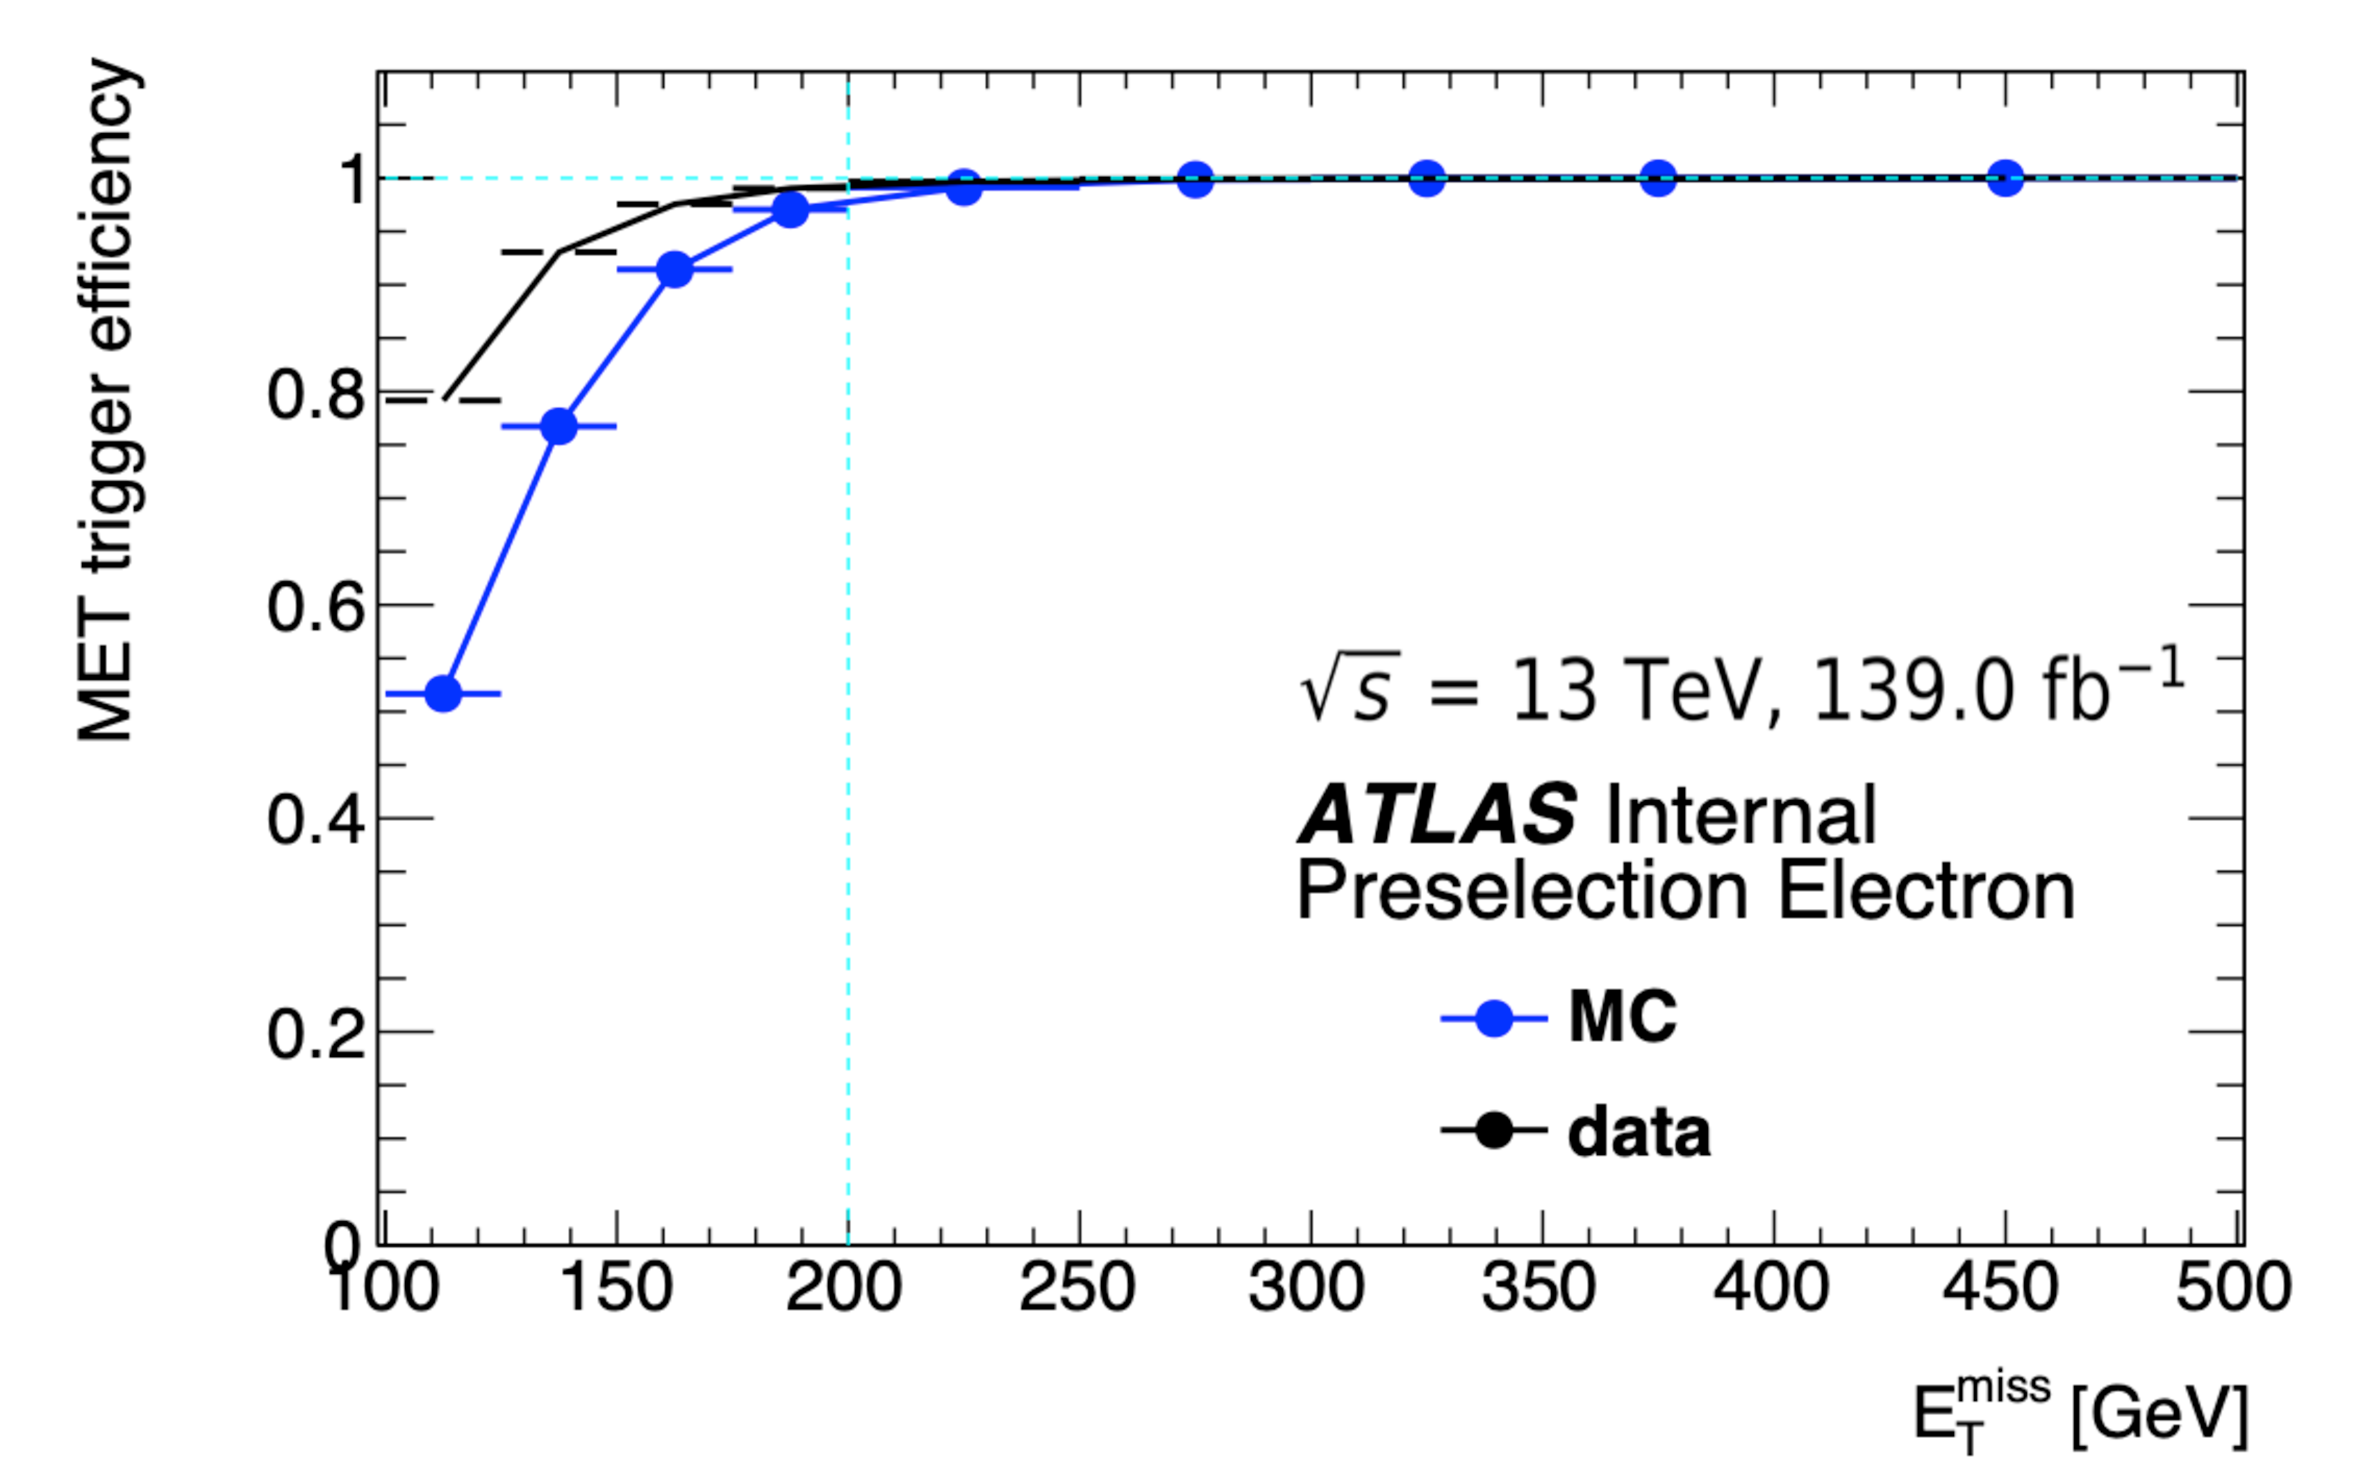
\includegraphics[width = 0.98\textwidth]{Figures/5/METTrigger/PreE_MetTST_met.pdf}
    \caption{Electron Channel}
    \label{ig:mettrig_e}
     \end{subfigure}
    \begin{subfigure}{0.49\textwidth}
     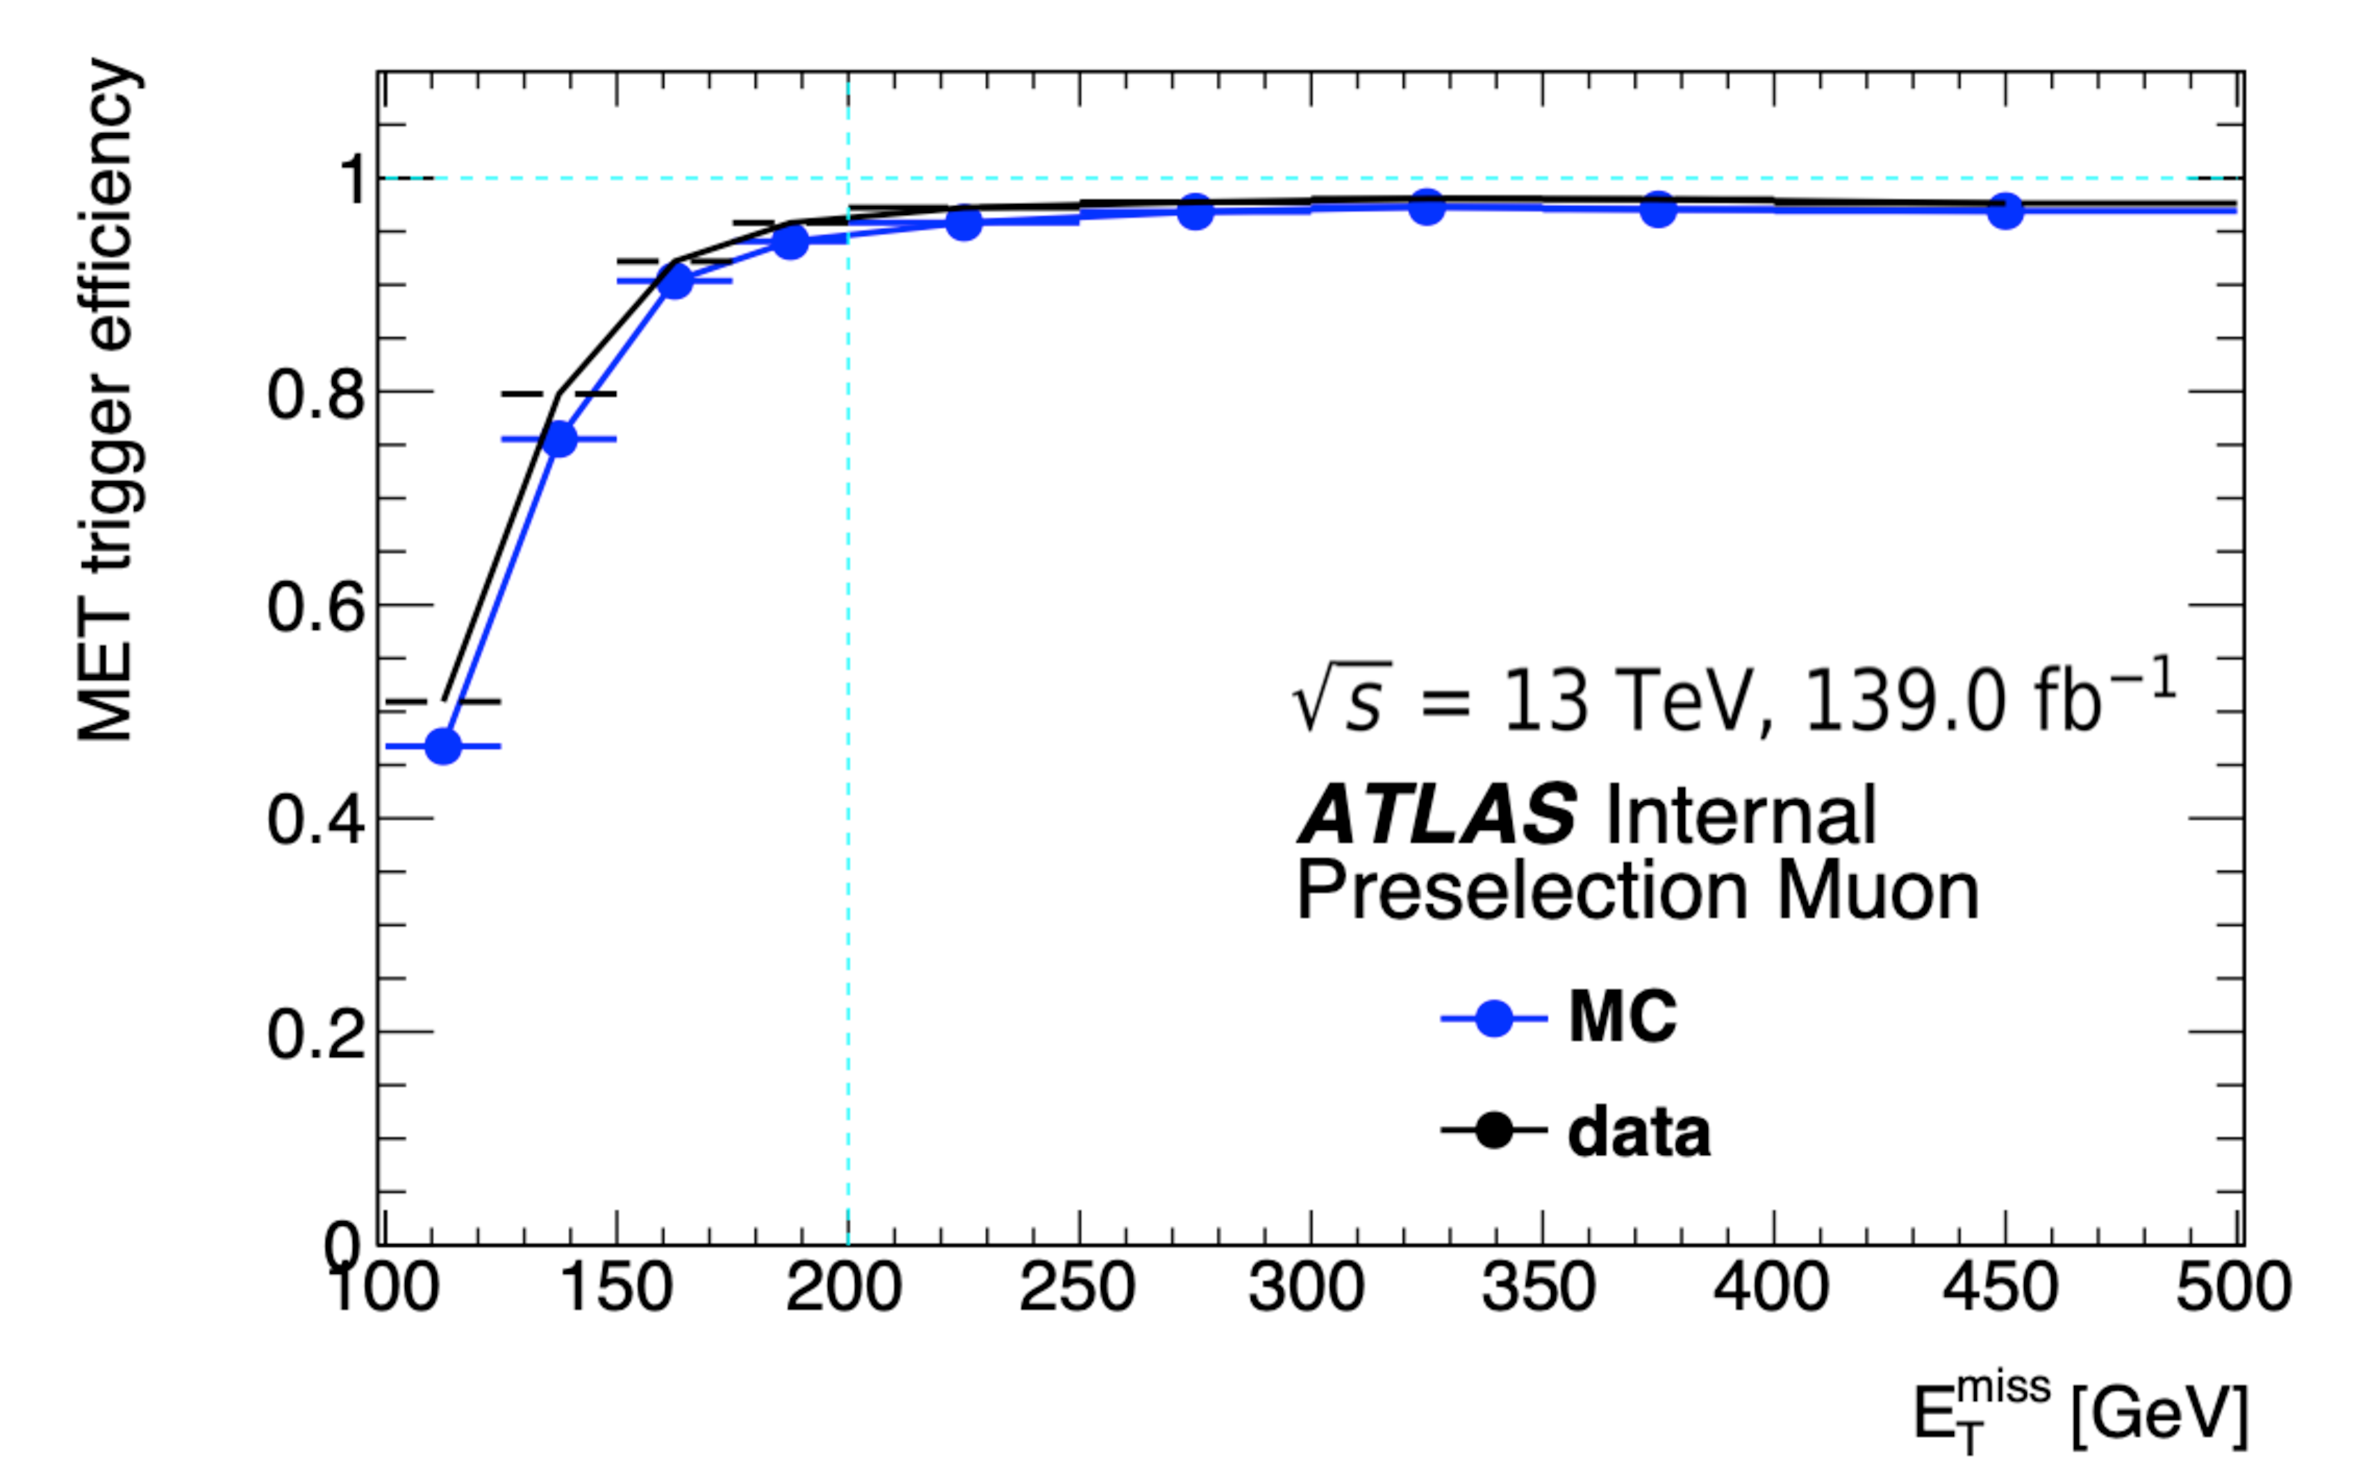
\includegraphics[width = 0.98\textwidth]{Figures/5/METTrigger/PreM_MetTST_met.pdf}
     \caption{Muon Channel}
     \label{ig:mettrig_mu}
     \end{subfigure}
     \caption{Comparison of the \met trigger efficiency defined in Eq. \ref{eq:met_trig_eff}, as a function of the \met lower bound in the event selection, between MC simulated events and ATLAS data in a region defined by a loosened baseline selection. The event selection is separated into electron (left) and muon (right) channels.}
     \label{fig:mettrig}
  \end{figure}
  
Comparing the trigger efficiencies in Figures \ref{fig:mettrig_e} and \ref{fig:mettrig_mu}, the efficiency in the electron channel converges to 100\% for \(\met > 200~\GeV\), but in the muon channel it instead converges to \(\sim90\%\) for \(\met > 200~\GeV\). After some investigation, the inefficiency in the muon channel was found to be due to events which have large \met arising from high-\pt muons. This is because high-\pt muons largely pass through the ATLAS calorimeter and are detected instead by the muon spectrometer. As a result, such high-\pt muon events can be missed by the \met triggers, which don't make use of information from the muon spectrometer \cite{met_performance_2019}. This can be seen by plotting the \met trigger efficiency using a calculation of \met in the event selection that ignores the muon \pt (a.k.a. ``muon invisible") in Figure \ref{fig:metmuinvis}, and observing that in this case the efficiency converges to 100\% for \met (muon invisible) \(> 200~\GeV\). 

\begin{figure}[htbp]
    \centering
     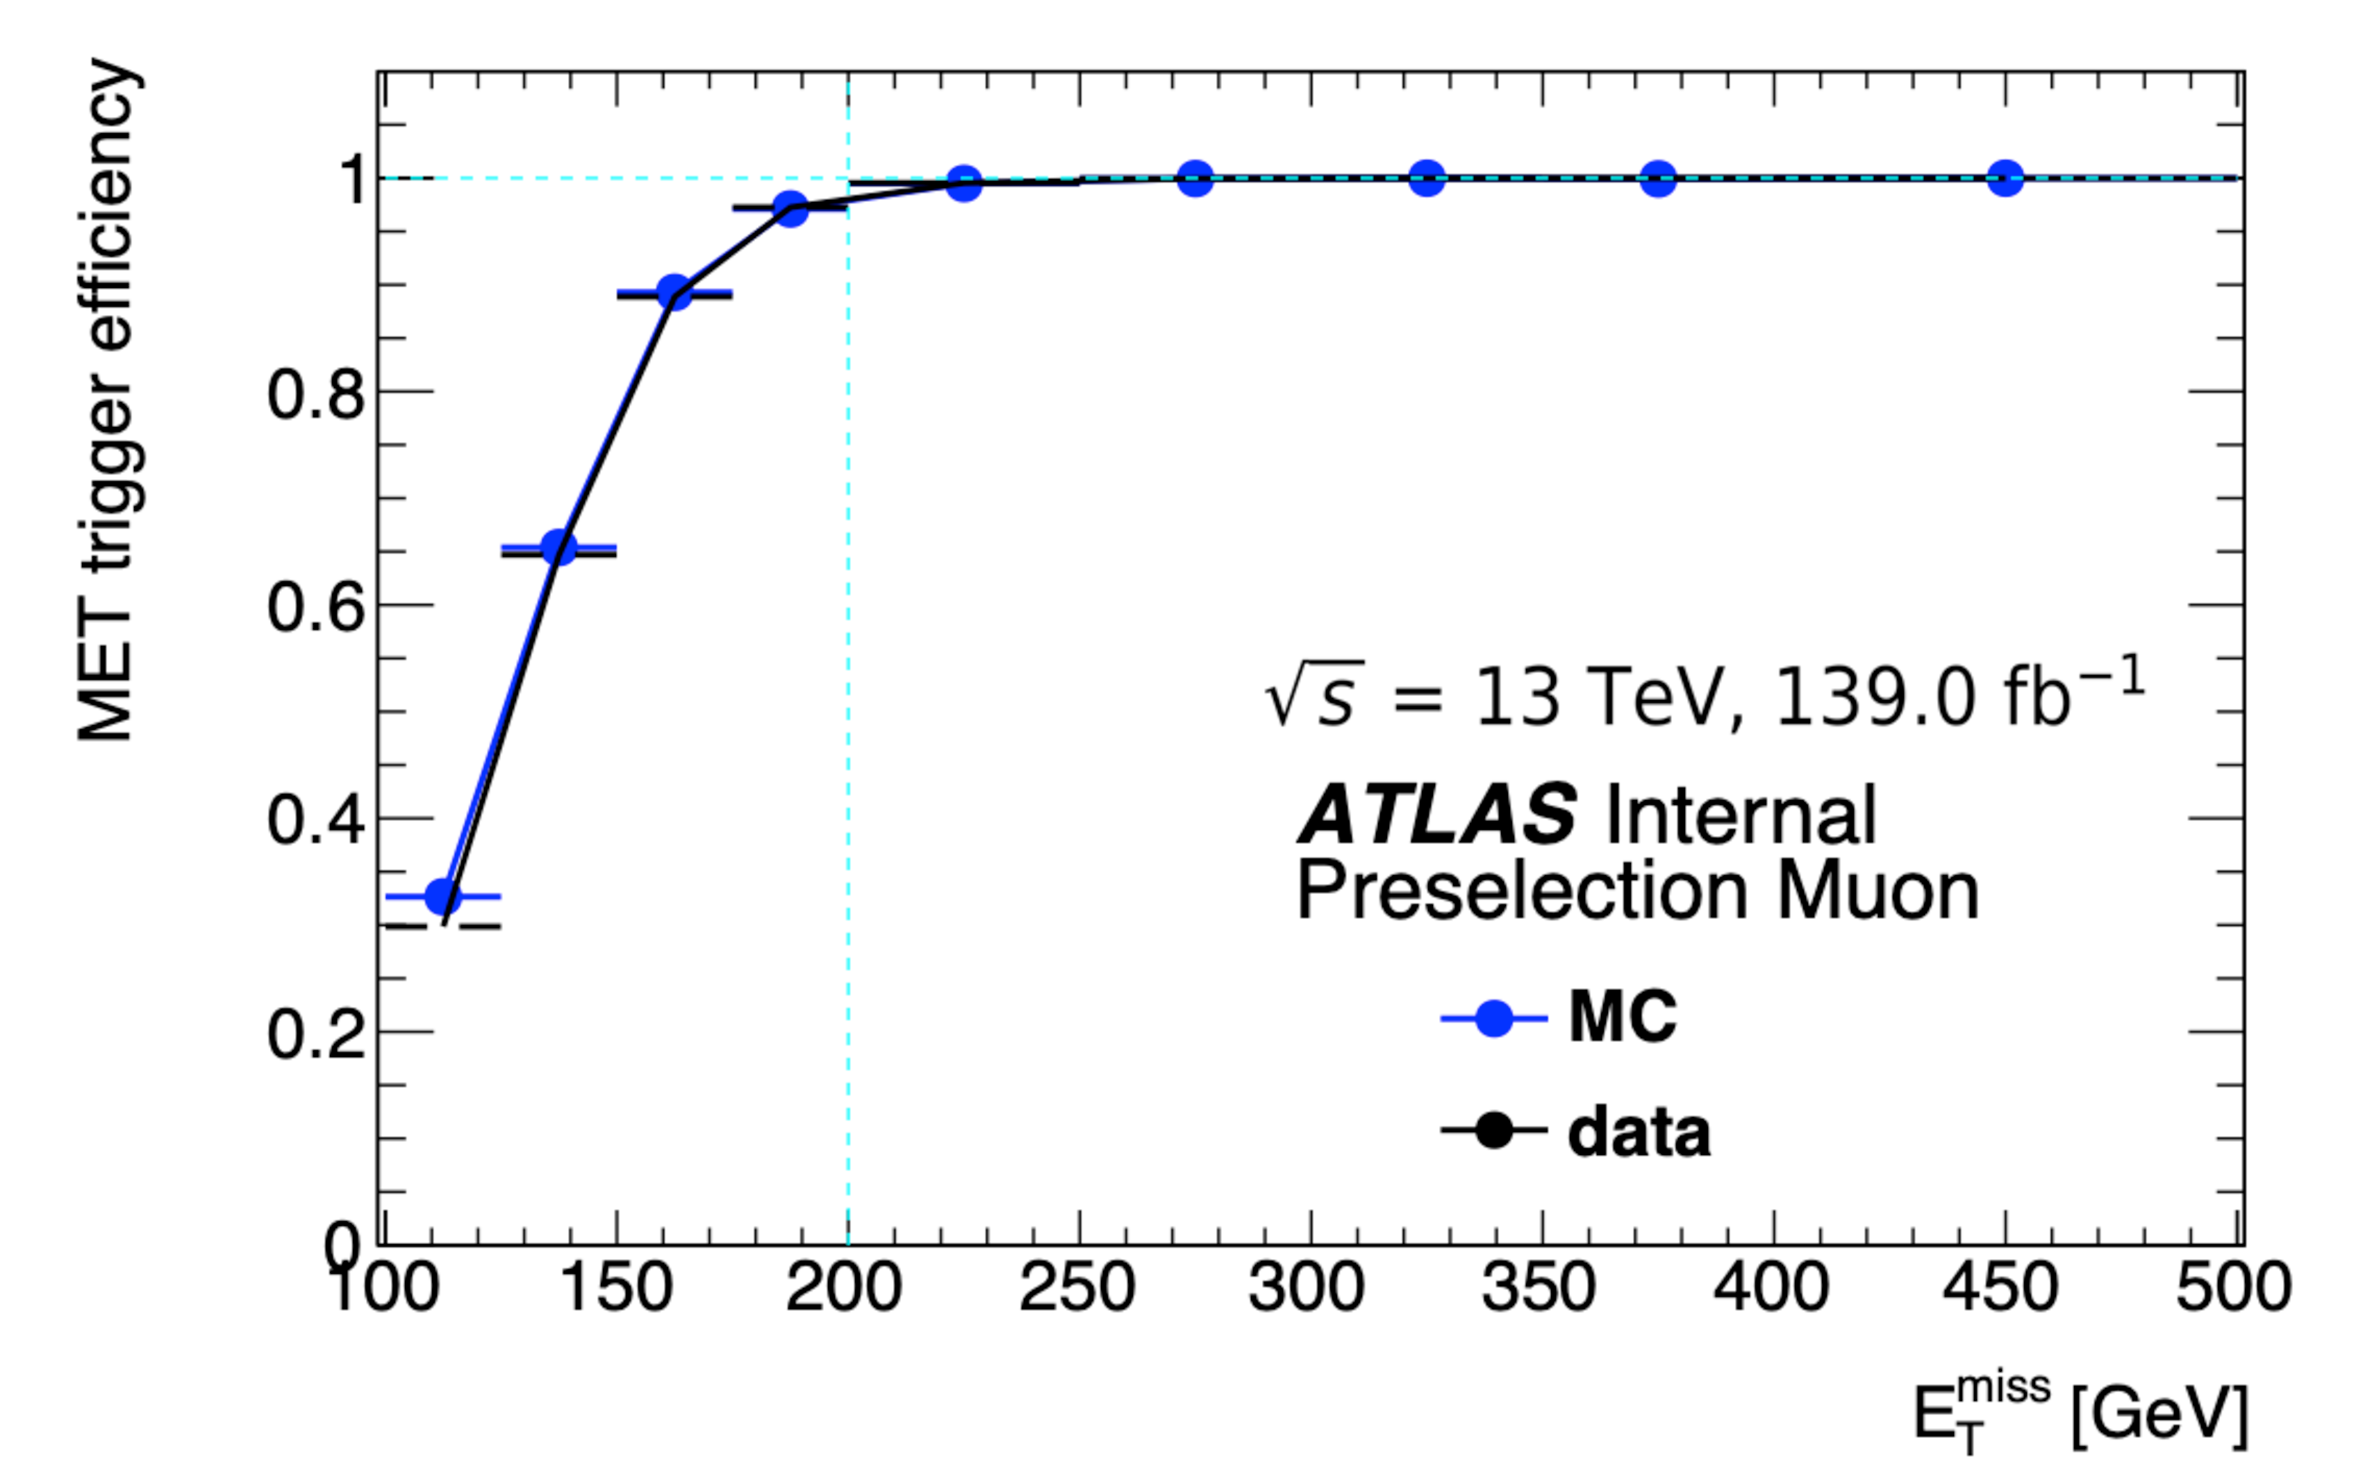
\includegraphics[width = 0.6\textwidth]{Figures/5/TriggerMuInvis/Pre_MetTST_met.pdf}
     \caption{\met trigger efficiency, as a function of the \met lower bound for the loosened baseline event selection in the muon channel, with muons treated as invisible in the calculation of \met}
     \label{fig:metmuinvis}
  \end{figure}
 
As discussed above, events which pass the baseline selection in the muon channel with \(\met > 200 ~\GeV\) but fail the \met trigger generally have large muon \pt. It was found that these high-\met events in the muon channel which fail the \met trigger do, however, pass the muon trigger with high efficiency. For this reason, the efficiency of a logical OR of the \met and single muon triggers is studied in the muon channel. This \met or single muon trigger efficiency is calculated as follows for MC simulated events for a given set of event selection criteria which define a region ``X":

\begin{equation}
\label{eq:met_or_single_muon_trig}
\begin{footnotesize}
\text{eff}_\text{\met OR single muon, MC, region X} = \frac{\sum_i w_i\text{ passing ($\met$ OR single muon triggers)\text{ AND }(in region X)}}{\sum_i w_i\text{ in region X}}
\end{footnotesize}
\end{equation}

\noindent where the event weight \(w_i\) in the numerator includes the scale factors to correct for the known \(<100\%\) trigger efficiency of the single muon trigger. Note that since Eq. \ref{eq:met_or_single_muon_trig} is evaluated only for MC simulated events, there is no need for an independent trigger in the numerator and denominator such as the single lepton trigger included in Eq. \ref{eq:met_trig_eff}. As shown in Figure \ref{fig:trigger_OR}, the \met OR single muon trigger is found to be effectively 100\% efficient, given the application of appropriate scale factors for the single muon trigger, in the muon channel with the loosened baseline event selection for all lower bounds on the \met down to  \(\sim 100~\GeV\).

  \begin{figure}[htbp]
  \centering
    \begin{subfigure}{0.49\textwidth}
     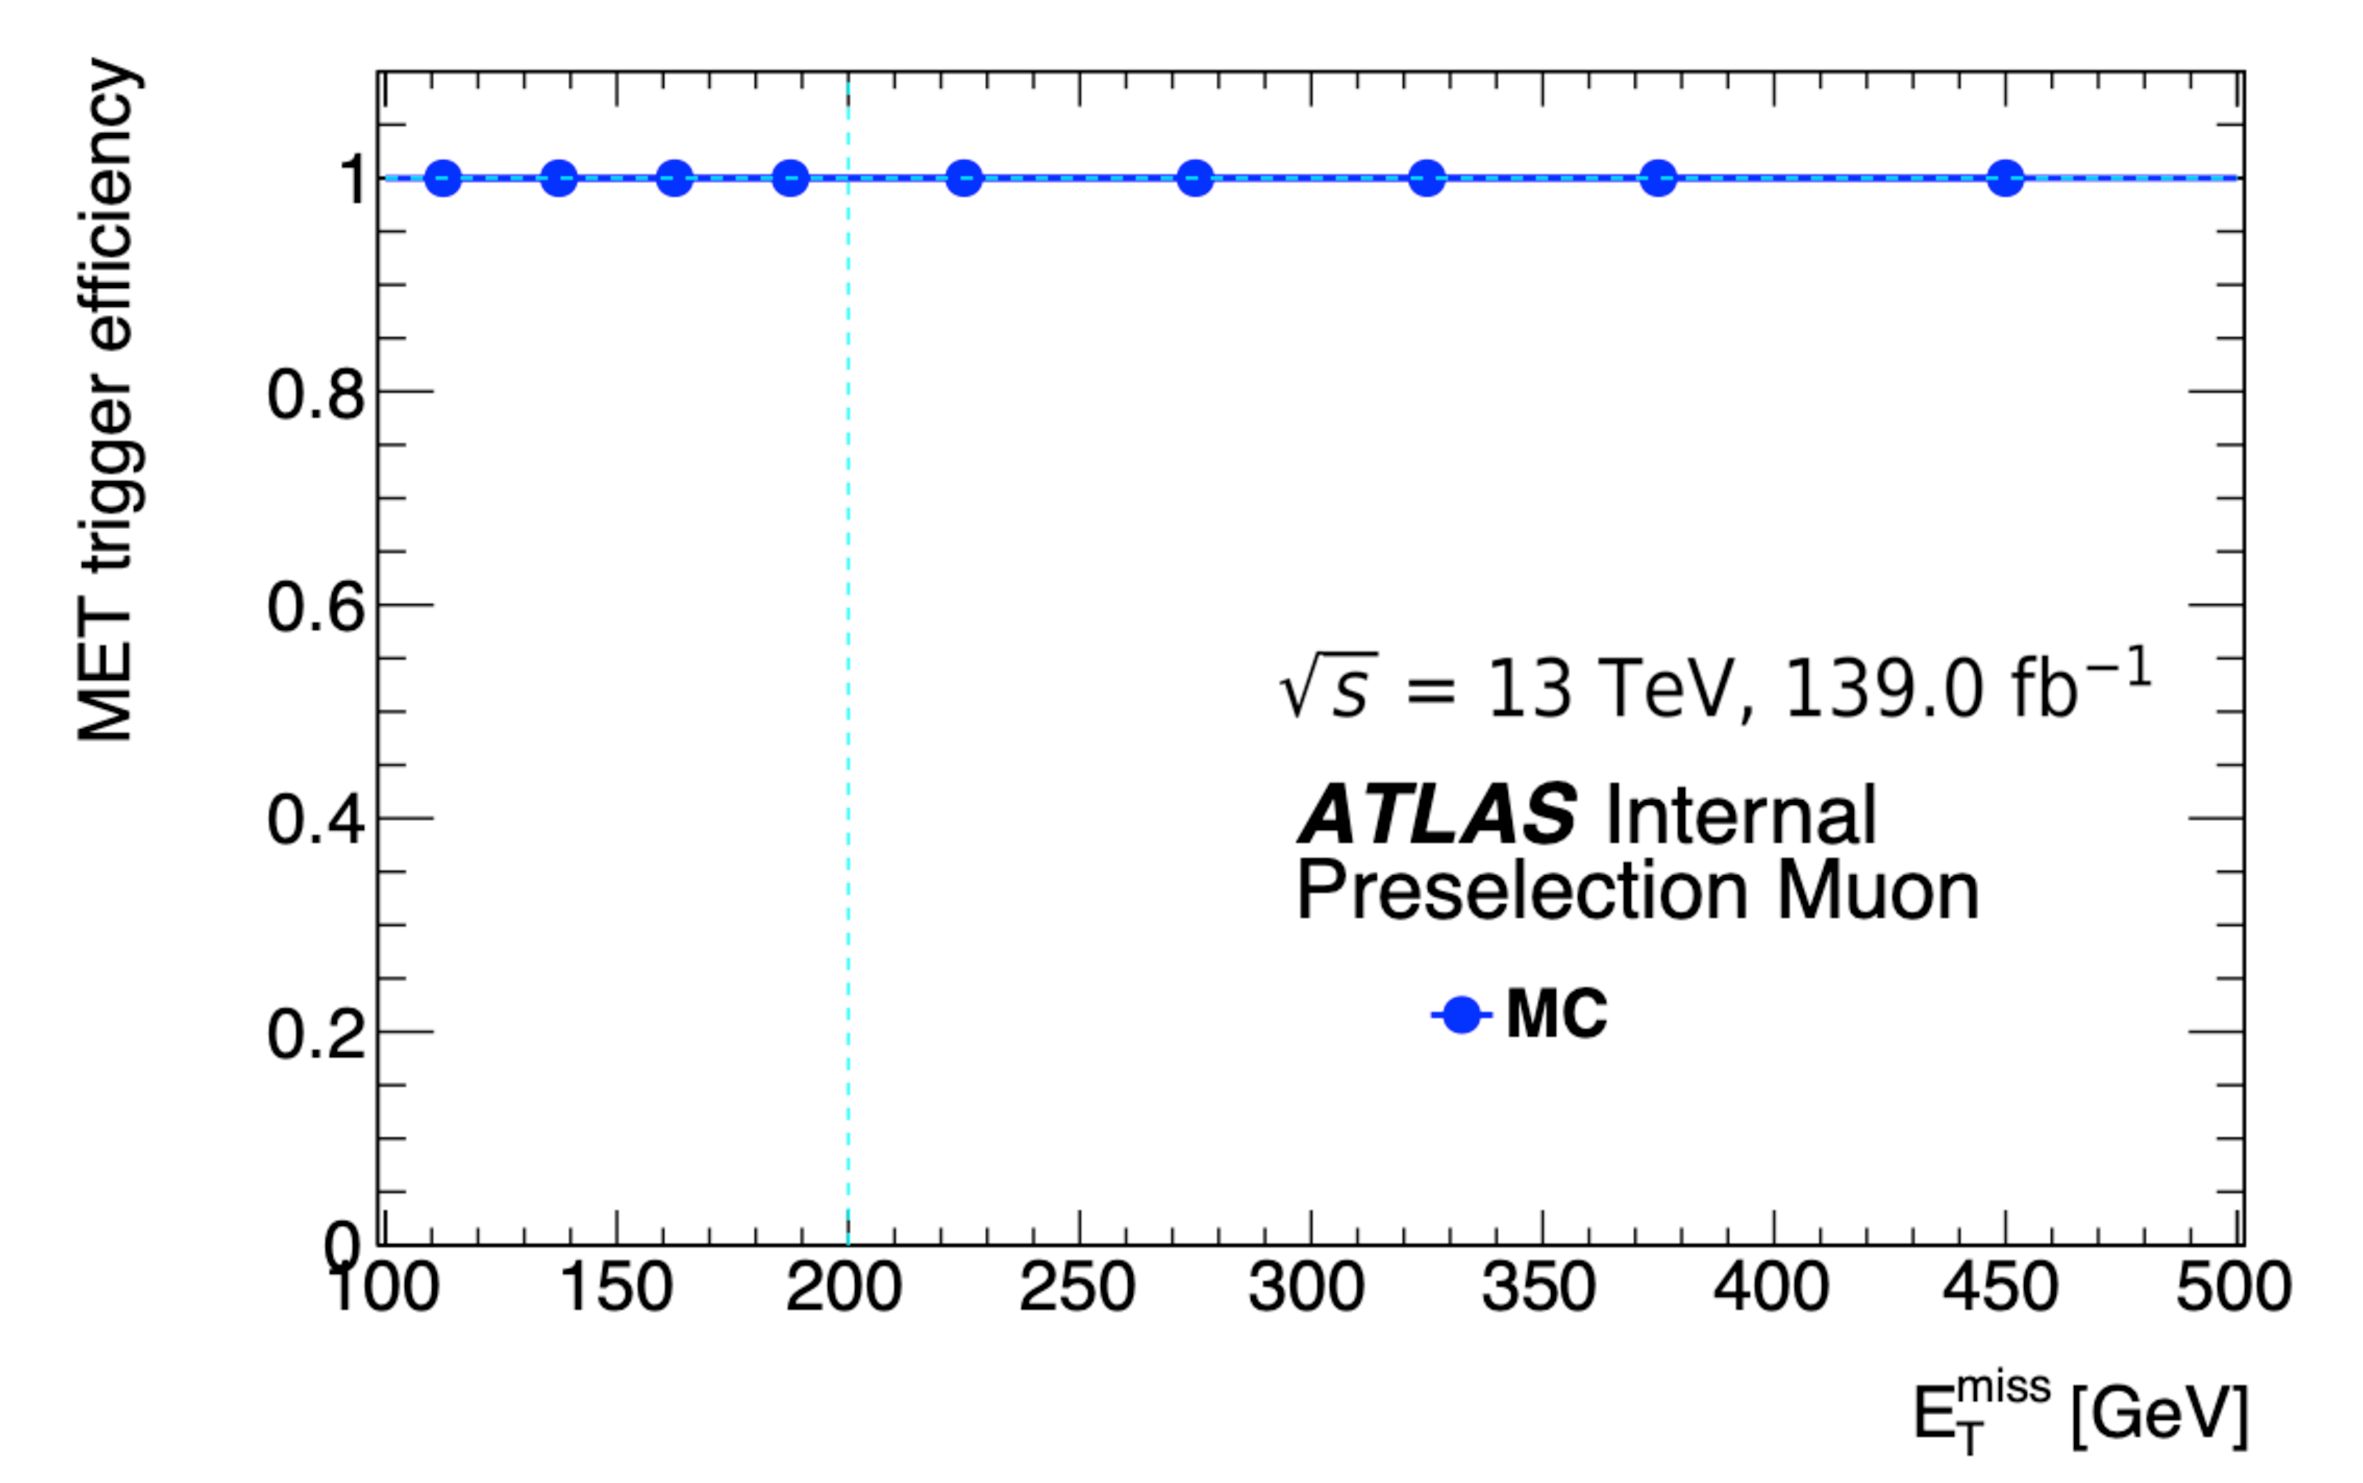
\includegraphics[width = 0.98\textwidth]{Figures/5/TriggerOR/Pre_MetTST_met.pdf}
     \caption{Preselection}
     \end{subfigure}
     \caption{Efficiency of the \met OR single muon trigger, as a function of the \met lower bound, in the muon channel for the loosened baseline event selection in the muon channel.}
     \label{fig:trigger_OR}
  \end{figure}

Based on the analysis presented in this section, it is concluded that, if all events considered in the analysis are explicitly required to have passed the \met or the single muon trigger, the trigger efficiency is known to be 100\% for all events except for the small subset of events with a high-\pt muon which pass the muon trigger but fail the \met trigger. For these events, scaling factors and associated uncertainties, which are determined by independent calibrations performed by the ATLAS collaboration, are included in the event weight to correct for the known \(<100\%\) efficiency of the single muon trigger. An additional ``trigger-matching" requirement is applied for events which fail the \met trigger but pass the single muon trigger. This trigger matching requires that the final state muon object that was reconstructed during data-taking and which activated the single muon trigger can be identified as the same muon object (i.e. as having originated from the same muon) that was later reconstructed with the more granular offline reconstruction software. 
